\documentclass[10pt]{beamer}

\IfFileExists{/home/torterotot/Documents/PhD-Thesis/README.md}{\def\PhDthesisdir{/home/torterotot/Documents/PhD-Thesis}}{}
\IfFileExists{/home/lucas/Documents/PhD-Thesis/README.md}{\def\PhDthesisdir{/home/lucas/Documents/PhD-Thesis}}{}

\IfFileExists{/home/lucas/texmf/tex/latex/ltstyle/ltstyle.sty}{\def\homedir{/home/lucas}}{}
\IfFileExists{/home/torterotot/texmf/tex/latex/ltstyle/ltstyle.sty}{\def\homedir{/home/torterotot}}{}
\RequirePackage[log-declarations=false]{xparse}
\usepackage[english]{babel}
\usepackage[none,Roboto,beamerheader,beamerlogo]{ltstyle}
\addbibresource{\PhDthesisdir/bib/Bibliographie_PhD_Torterotot.bib}
\usecolortheme[named=CERNblue]{structure} 

\institute[IP2I]{Institut de Physique des deux Infinis -- Lyon} % Lycée Kléber  Lycée Assomption Bellevue ... possède une version courte optionnelle
\title{Recherche d'un boson de Higgs de haute masse se désintégrant en paire de taus dans l'expérience CMS au LHC}
\matiere{Thèse de doctorat}
\author{Lucas \textsc{Torterotot}, Colin \textsc{Bernet}}
\date{\todo{XX xxxx} 2021}

%\AtBeginDocument{\setbeamertemplate{footline}{\vskip0pt}}
%\AtBeginDocument{\setbeamertemplate{headline}{\leavevmode}}

%\AtBeginSection[]{\begin{frame}<beamer>\addtocounter{framenumber}{-1}\tableofcontents[currentsection,currentsubsection]\end{frame}}
%\AtBeginSubsection[]{\begin{frame}<beamer>\addtocounter{framenumber}{-1}\tableofcontents[currentsection,currentsubsection]\end{frame}}
%\AtBeginSubsubsection[]{\begin{frame}<beamer>\addtocounter{framenumber}{-1}\tableofcontents[currentsection,currentsubsection,currentsubsubsection]\end{frame}}

%\setbeamertemplate{navigation symbols}{%items présents dans la barre de navigation
%\insertslidenavigationsymbol
%\insertframenavigationsymbol
%\insertsubsectionnavigationsymbol
%\insertsectionnavigationsymbol
%\insertdocnavigationsymbol
%\insertbackfindforwardnavigationsymbol
%}

\newcommand{\graphh}{0.8\textheight}
\newcommand{\graphw}{\textwidth}
\newcounter{totalframes}

\IfFileExists{\homedir/Dropbox/resources/img/logos/CERN/CERN-logo_bleu.jpg}{
\def\upperleftlogos{
\includegraphics[height=.5cm]{\homedir/Dropbox/resources/img/logos/CERN/CERN-logo_bleu.jpg}\quad
\includegraphics[height=.5cm]{\homedir/Dropbox/resources/img/logos/CMS/CMSlogo_white_nolabel_128_May2014.png}}
\def\upperrightlogos{
\includegraphics[height=.5cm]{\homedir/Dropbox/resources/img/logos/IN2P3/IN2P3Filaire-B_SignV_noirNB-eps-converted-to.pdf}\quad
\includegraphics[height=.5cm]{\homedir/Dropbox/resources/img/logos/IP2I/logo_IP2I.jpg}}
\def\lowerleftlogos{}
\def\lowerrightlogos{}
}{}

\begin{document}
\IfFileExists{\homedir/Dropbox/resources/img/logos/CERN/CERN-logo.jpg}{
\begin{frame}[noframenumbering] \thispagestyle{empty}
\vspace{-.75cm}


\includegraphics[height=1.25cm]{\homedir/Dropbox/resources/img/logos/Gouvernement/ES-R-I_horizontal.pdf}
\hfill

\includegraphics[height=1.25cm]{\homedir/Dropbox/resources/img/logos/ED52-PHAST/phast-logo.png}
\hfill

\includegraphics[height=1.25cm]{\homedir/Dropbox/resources/img/logos/UCBL/Planche_UdL_LogoLyon1Sig_CoulCmjnVecto-eps-converted-to.pdf}

\vfill

\titlepage

\vfill

~ \hfill

\includegraphics[height=1.25cm]{\homedir/Dropbox/resources/img/logos/IN2P3/IN2P3-B_SignV_bleu-eps-converted-to.pdf}
\hfill

\includegraphics[height=1.25cm]{\homedir/Dropbox/resources/img/logos/CERN/CERN-logo.jpg}
\hfill
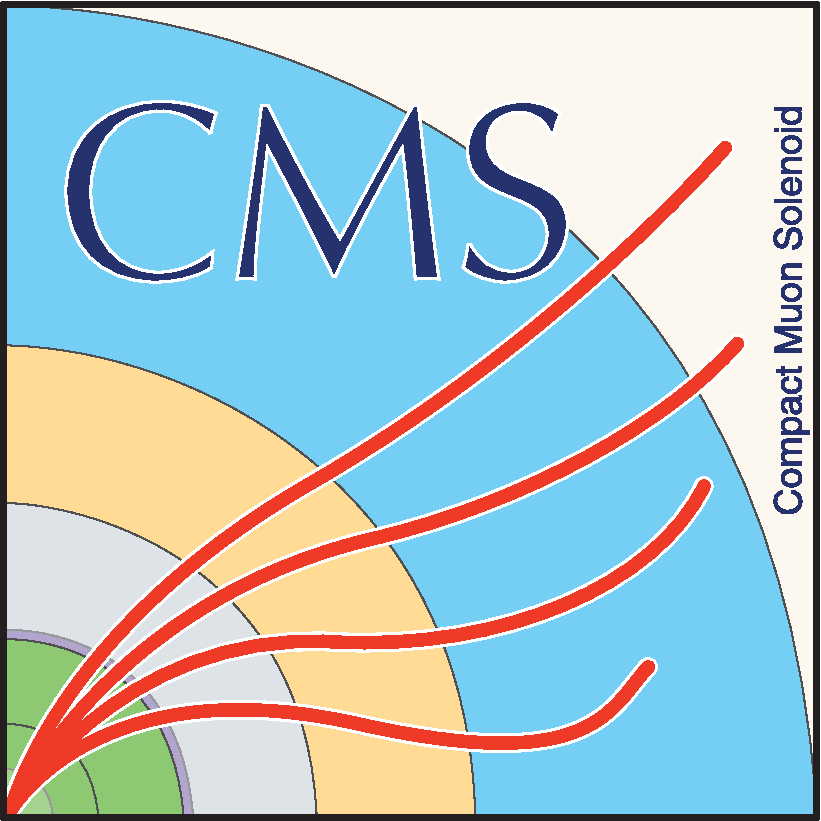
\includegraphics[height=1.25cm]{\homedir/Dropbox/resources/img/logos/CMS/CMS_logo.pdf}
\hfill

\includegraphics[height=1.25cm]{\homedir/Dropbox/resources/img/logos/IP2I/logo_IP2I.jpg}
\hfill ~

\vspace{-.5cm}
\end{frame}
}{
\begin{frame}[noframenumbering] \thispagestyle{empty}
\titlepage
\end{frame}
}

\begin{frame}
\tableofcontents 
\end{frame}


\begin{frame}\thispagestyle{empty}
\begin{center}
{\large \color{CERNblue}{Thank you for your attention!}}

\vspace{.25\textheight}
\end{center}
\end{frame}

\setcounter{totalframes}{\theframenumber}

%%% backup 

\setcounter{framenumber}{\thetotalframes}

\end{document}
